\chapter{Supertagging}
\label{chapter:sup}
This chapter is an extended version of~\cite{constructive}, to be presented in the fourth workshop on Representation Learning for NLP (REPL4NLP).

\section{Background}
The extraction algorithm, as described in Chapter~\ref{chapter:extraction}, produces a type-annotated DAG.
Projecting a DAG's yield we obtain a sentence where each word is decorated with its corresponding type, which is the minimal information required to begin a proof-theoretic analysis of the sentence.
Obviously, a system only capable of analyzing sentences that it has already been exposed to is of little practical use.
The question then naturally arises of how to enable analyses for sentences not contained in the original corpus.
The answer is supertagging~\cite{supertagging}; a process that employs statistical learning techniques to probabilistically model the type assignment process.
In what follows, we will inspect supertagging, as initially introduced, gradually expanding the original formulation with additional components that broaden its applicability, alongside the literature that introduced them. 
For each such component, a paragraph will be devoted to motivating our reasons for incorporating such additions with reference to our data and the current problem specification.
Regardless of the particular implementation, the common point lies in the treatment of the type-annotated corpus as a training dataset. 
The corpus is treated as a collection of information-carrying samples, which may be used for inferring the parameters of a statistical model (of varying complexity).
The hypothesis is that, after parameter tuning, the trained model can be general enough to correctly analyze new sentences.

\subsection{Original Formulation}
To set things off, we may define $\mathcal{T}$ as the set of types assigned by the extraction process.
First, recall that each word occurrence is assigned a corresponding type.
However, not all occurrences of the same word are necessarily assigned the same type.
A sensible approach is to then view the extraction's output as a type lexicon $\mathcal L$, a mapping that sends each word of the input vocabulary $\mathcal{V}$ to a probability distribution over types:
\[
\mathcal{L}: \mathcal{V} \to \mathcal{S}^{|\mathcal{T}|}
\]
where $\mathcal{S}^{|\mathcal{T}|}$ refers to the standard $|\mathcal{T}|$-simplex, such that:
\[
\mathcal{L}(w) = \left \{ \frac{o(w, \tau)}{\sum_{t \in \mathcal{T}}{o(w, t)}} \ \forall \ \tau \in \mathcal{T} \right \} 
\]
where $o(w, \tau)$ simply counts the number of times word $w$ has occurred with type $\tau$.

This definition of a type lexicon is completely faithful to its original formulation by Bangalore and Joshi.
Although illuminating as a starting point, it suffers from a number of limitations.
Several of those have already been addressed by prior work, and the next subsections are devoted to explaining how.

\subsection{Unbounded Domain}
Our treatment of the lexicon as a mapping from a prespecified vocabulary inherently fails to address type-assignment for words not present in the training corpus.

\paragraph{Word Embeddings}
At this point, we will need to take a short detour to briefly introduce word vectors.
Word embeddings are dense, finite-dimensional vectorial representations that capture word semantic content. 
They inherit their functionality in virtue of the distributional hypothesis, which states that words with similar meanings exhibit similar use (i.e. they tend to appear under similar contexts).
The contextual surroundings of words may be statistically modelled using large-scale corpora in an unsupervised manner; the resulting distributions are high-dimensional and sparse.
Word vectorization techniques are applied on top of these, producing low-dimensional, dense representations.
This may be accomplished either in a predictive manner (e.g. fit the parametric representations of words so as to predict a missing word given its context) or as simple factorizations of the input (e.g. perform singular-value decomposition on the co-occurrence matrix).
Generally speaking, word vectorization techniques accept large, unstructured textual input and produce a vector space with implicit but rich topological structure. 
Words are assigned vectors within that space, and linguistic notions are inherited in the form of numeric operations, with the prime example being semantic similarity between words materializing as angular distance between vectors.
With the recent advent of neural networks, word vectorization techniques have risen in popularity and efficiency, achieving impressive results in encoding both syntactic and semantic information.

\paragraph{Domain Expansion}
Given that word embedding algorithms require no structured input, they may be trained on corpora scales of magnitude larger than the extraction algorithm, therefore containing many more words.
Let $\mathcal{E}$ be a word embedding system, trained on a corpus with vocabulary $\mathcal{V}'$, where $\mathcal{V}' \supset \mathcal{V}$, that produces vectors in a $d$-dimensional space:
\[
\mathcal{E}: \mathcal{V}' \to \mathbb{R}^d
\]
Then, we may use our lexicon $\mathcal{L}$ to parametrically fit a continuous function $f_\mathcal{L}: \mathbb{R}^d \to \mathcal{S}^{|\mathcal{T}|}$, which by function composition yields a probabilistic lexicon over an expanded domain:
\[
 f_\mathcal{L} \circ \mathcal{E}: \mathcal{V}' \to \mathbb{R}^d
\]


\paragraph{Domain Unbounding}
The above addition allows expanding the supertagger's domain to words not present in the type-annotated corpus.
Language is not a closed construct, however; there still is a possibility of the supertagger encountering a word $w$ that is not present in the expanded corpus.
Rather than backing to default behavior, a further and final expansion of the domain may be achieved by incorporating sub-word information (e.g. morpheme- and character-level content).
In fact, modern vectorization techniques do utilize such information in order to account for languages that feature word generation by compounding or rich but systematic morphology~\cite{fasttext}.
Then, $\mathcal{E}$ becomes a mapping from any word in the language $L$ onto an object of the vector space:
\[
\mathcal{E}: L \to \mathbb{R}^d
\]
and its composition with the continuous type-assignment function is an unbounded domain supertagger:
\[
f_\mathcal{L} \circ \mathcal{E}: L \to \mathcal{S}^{|\mathcal{T}|}
\]

\paragraph{Case In Point}
The practical importance of achieving the maximal possible expansion of the supertagger's domain is substantiated by our corpus' statistics; the extraction output contains little over 73\,000 unique words, whereas the Woordenboek der Nederlandsche Taal (Dictionary of the Dutch Language)\cite{woordenboek} contains approximately 400\,000.

\subsection{Type Disambiguation}
The next thing to address is the ambiguity of the type assignment process.
As pointed out in the original supertagging proposal, the fact that lexical items are assigned different types for each syntactic context they appear in comes at the cost of local ambiguity that needs to be resolved for accurate parsing.

In order to reduce it (or even completely eliminate it), we may inform the type assignment function with surrounding context $\mathcal{C}$:
\[
f_\mathcal{L}: \mathcal{L} \ \otimes \ \mathcal{C} \to \mathcal{S}^{|\mathcal{T}|}
\]
Our notion of context, and the means of representing it, can for now remain abstract as it varies between implementations.
Generally, the syntactic and semantic content of words is largely disambiguated by the surrounding words, so these are valid candidates for inclusion.
Similarly, the proof-theoretic behavior of types imposes certain constraints on the types they may interact with; therefore a formulation that iteratively assigns types while taking prior assignments into consideration is bound to benefit overall performance.

The first approaches to reducing ambiguity involved simple heuristics pertaining to the satisfiability of minimal structural constraints (e.g. the span of the annotation must fall within the sentence boundaries), or modeling joint probabilities over word-type pair spans.
During the later half of the last decade, recurrent networks rose to prominence in supertagging literature, owing to their general adoption as the de-facto computational machinery for sequential processing, as well as the increased availability of high-quality word vectors.
~\cite{xu-etal-2015-ccg} first applied a simple recurrent network~\cite{elman1990finding} for CCG supertagging, whereas~\cite{lewis-etal-2016-lstm} and~\cite{vaswani-etal-2016-supertagging} utilized bi-directional Long Short-Term Networks~\cite{hochreiter1997long}, each successively achieving higher performance benchmarks.
In their general formulation, such systems accept as their input a sequence of vectors representing a sentence, and apply a recurrent function on them, tasked with producing contextually aware feature vectors.
The latter are then used to model each word's class membership over supertags, turning the problem into an instance of sequence labeling, a common case of supervised learning~\cite{graves2012supervised}.

\paragraph{Case In Point}
The fine-grained nature of our type system results in a large number of unique supertags, each characterizing a very specific phrasal structure.
On one hand, this means that words that uniformly assume a single syntactic role are highly likely to be assigned a single type.
On the other hand, words that exist in a broader range of contexts are increasingly ambiguous, even when these contexts are similar.

In practical terms, Figure~\ref{fig:type_ambiguity} displays a log-log plot of type ambiguity. 
Words are, on average, assigned 1.8 unique types.
The majority of words (55\,000 and 75\% of the total) are unambiguous throughout the corpus.
The next most likely bin counts 17\,000 words (23\%) that have up to 10 different possible types. 
1\,000 words (1.4\%) are highly ambiguous, with up to 100 different types.
Finally, there are almost 30 lexical items (mostly function words, e.g. coordinators) which are extremely ambiguous, reaching up to 500 potential assignments.



\begin{figure}
    \centering
    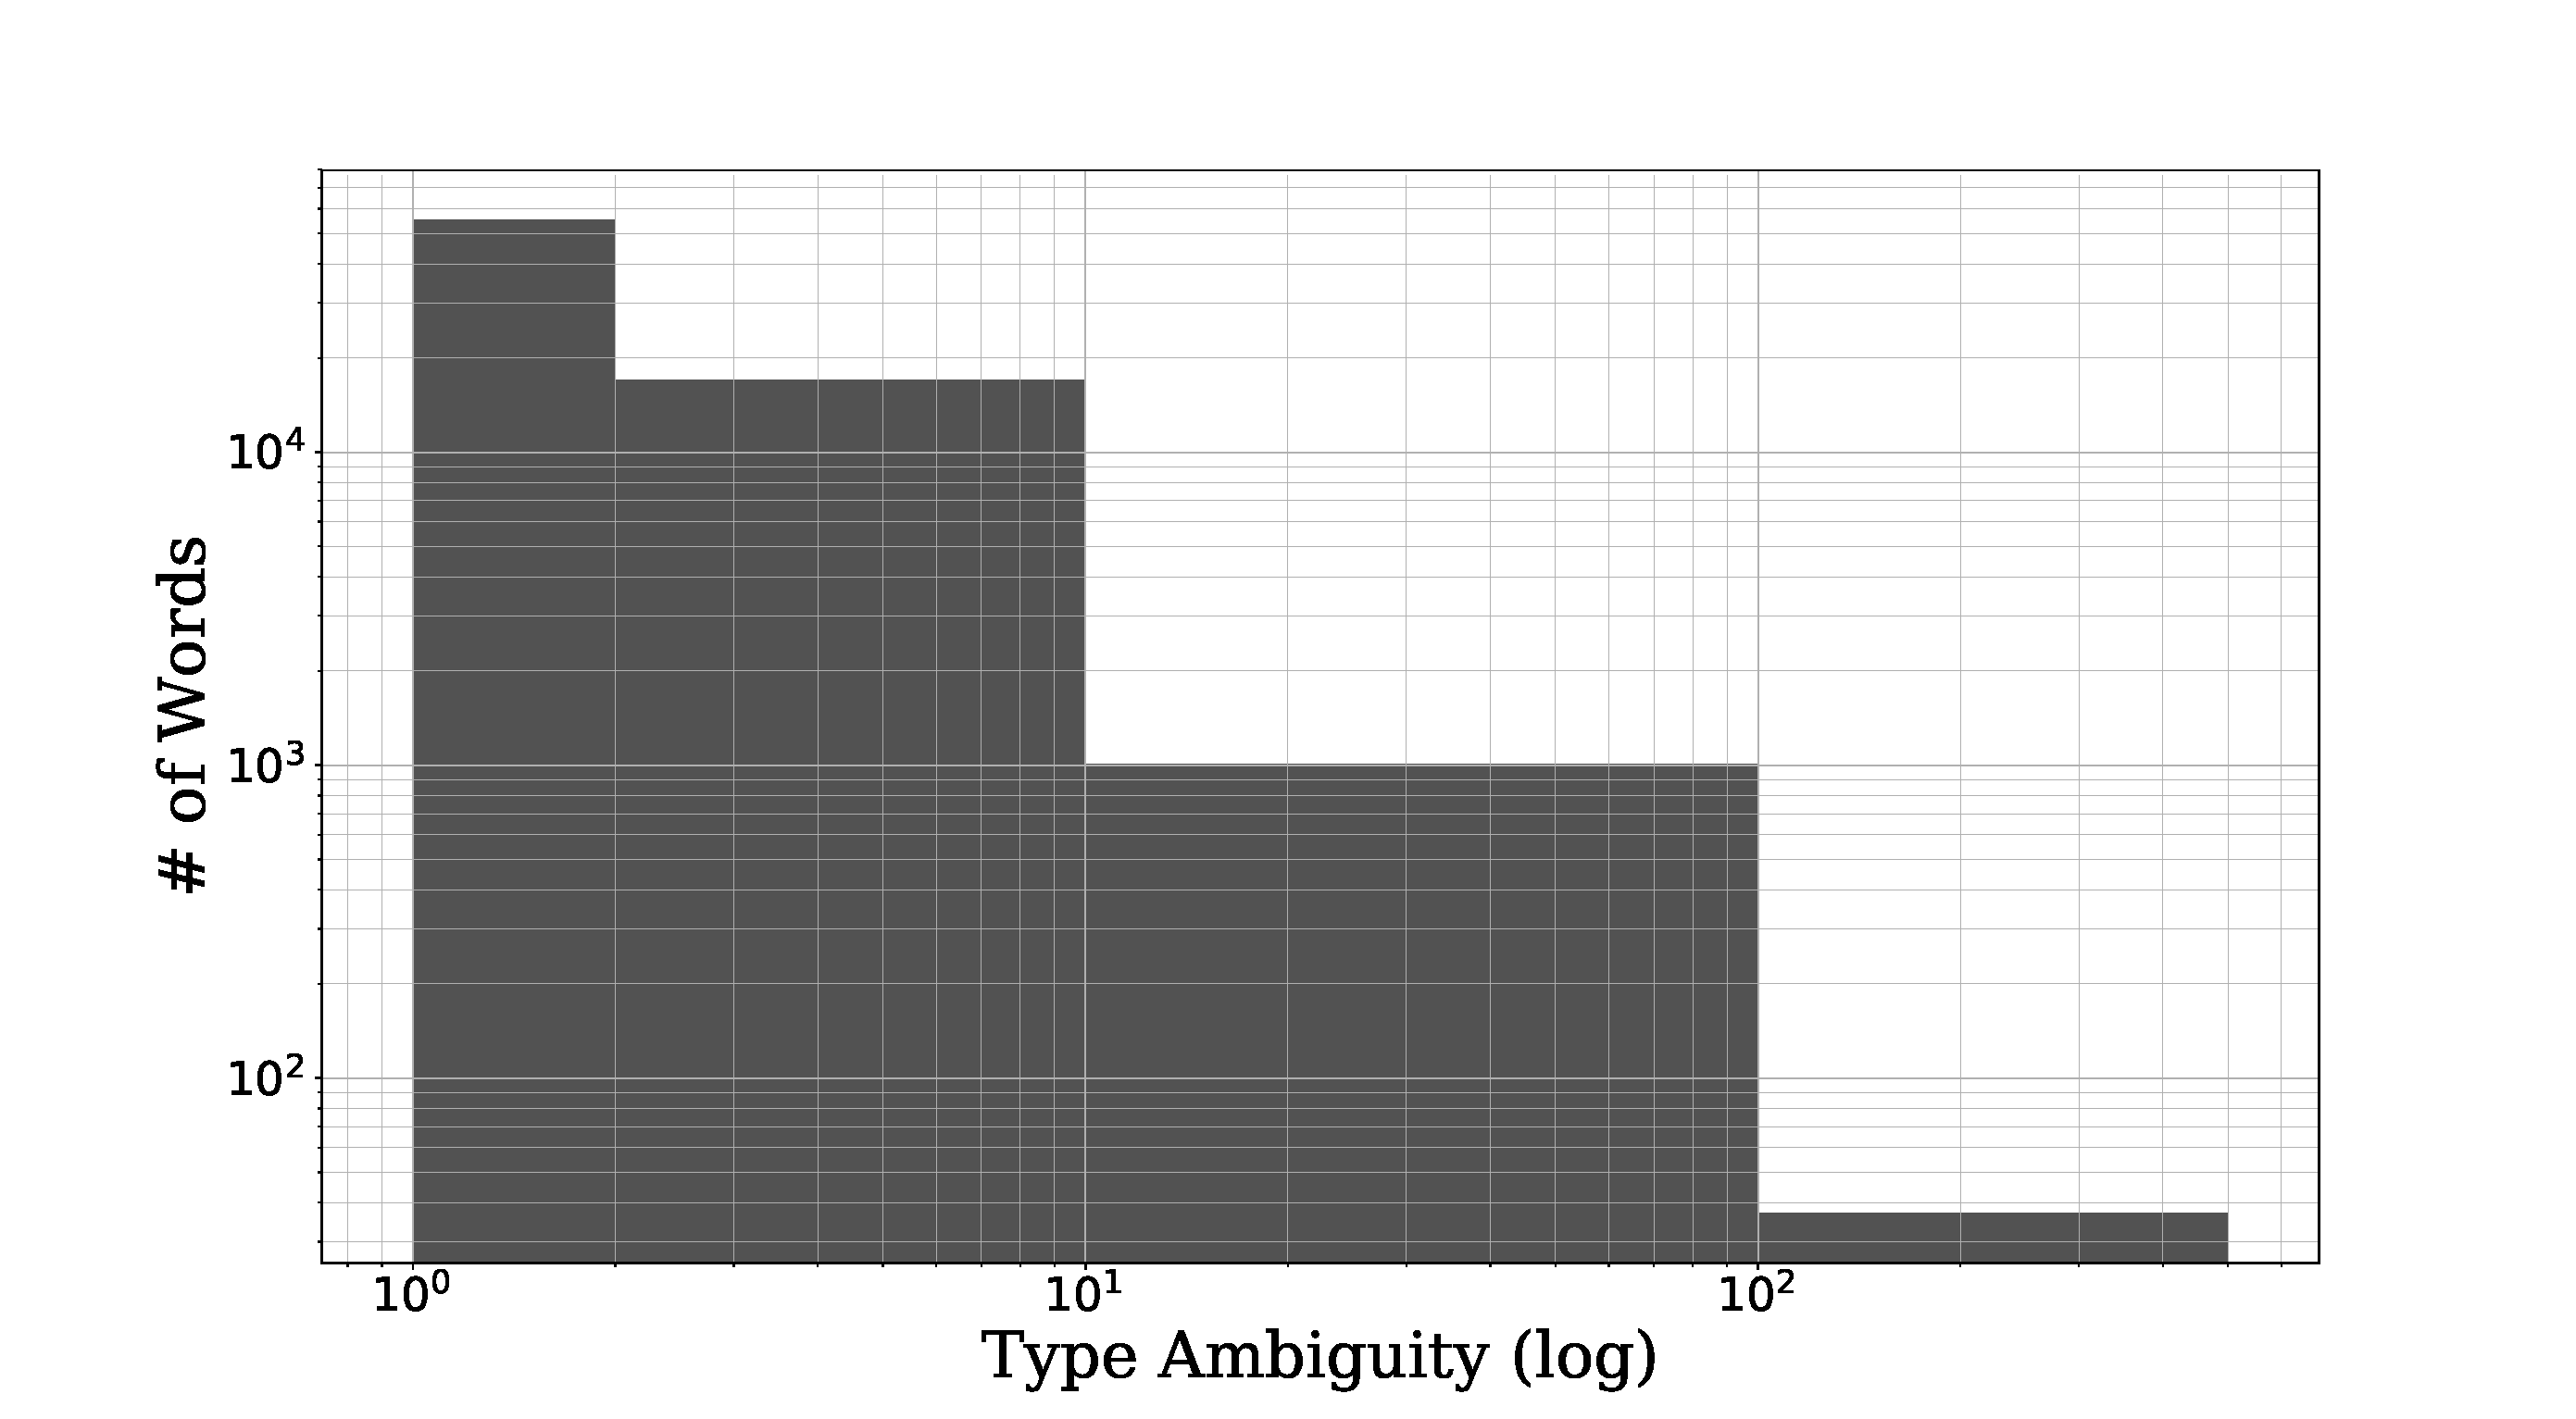
\includegraphics[scale=0.29]{Figures/ambiguity.pdf}
    \caption[Extracted Type Ambiguity]{Log-log bins of type ambiguity. The horizontal axis bins ranges of type ambiguity, and the vertical axis counts the number of unique lexical items that belong in each bin.}
    \label{fig:type_ambiguity}
\end{figure}

\section{Unbounded Codomain}
The previous section presented a brief overview of supertagging and its progress through the years.
It concluded with the current state of the art, which treats the problem as a case of sequence labeling, modeled by recurrent neural networks.
This perspective is quite natural, and allows supertagging systems to directly inherit the constant and ongoing progress of sequence labeling architectures.
These benefits, however, come at the expense of two significant side-effects, both inherent to classification algorithms.

The first pertains to the issue that class imbalance poses to supervised learners.
Across all categorial grammars, some categories have disproportionately low frequencies of occurrence compared to the more common ones, leading to severe sparsity issues, which are further pronounced the more refined the grammar is.
Under-represented categories are very hard to learn, especially in the context of sequence labeling, where under- and over-sampling are not immediately applicable.
As a result, modern supertagging models are commonly evaluated and tested against only small subset of the full categories present in a grammar, the elements of which have occurrence counts lying above a predetermined treshold.

Moreover, they operate under the strong assumption that the set of types that may be assigned is bounded, and also fully represented by the training corpus, i.e. known in advance.
Practically, the implicit hypothesis is that sentences that would require previously unseen supertags to be correctly analyzed do exist, but are sufficiently rare to be safely ignored.
Such a compromise might be realistic, but it still sets a fixed upper bound on the associated parser's strength.

Jointly, the above concessions have a far-reaching consequence; they place an implicit constraint on the nature of the grammars that may be learned.
Essentially, the grammar must be sufficiently coarse, allocating most of its probability mass on a small number of unique categories.
Grammars enjoying a higher level of analytical sophistication are virtually unusable, as to train an adequate supertagger for them would require prohibitive amounts of annotated data in order to overcome their sparsity.

Our grammar is one such, necessitating an alternative perspective.
This section is devoted to pointing out how a subtle reformulation of the problem bypasses the aforementioned limitations, allowing accurate supertagging with an unbounded codomain.

\subsection{The Language of Types}
Classification over an open set is a difficult problem undergoing active research.
Fortunately, even though our type vocabulary is open, its inhabitants are characterized by an important regularity.
They are all the made out of the same atomic components, the union of the sets of atomic types and $n$-ary logical connectives, each of which is itself closed.
Further, not all sequences of these components constitute valid types. 
Rather, all types are produced by a underlying inductive scheme:
\begin{align}
\textsc{t} ::= \ & \textsc{a} \ | \  \textsc{t}_1 \myrightarrow{\text{d}} \textsc{t}_2
\label{eqn:induction}
\end{align}
where $\textsc{t}$, $\textsc{t}_1$, $\textsc{t}_2$ are types, $\textsc{a}$ is an atomic type and $\myrightarrow{d}$ an implication arrow, decorated with the label $d$.

An examination of the above scheme reveals a simple context-free grammar (CFG).
Given the fact that our connectives are of fixed arity, the polish notation~\cite{hamblin1962translation} can be adopted, abolishing the need for parentheses and reducing the representation length of types, while also encoding their order in a succinct, up-front manner.
Then, the grammar materializes using just two meta-rules for productions:
\begin{align}
\{ (S & \implies A) \  \forall \ A \in \mathcal{A} \}
\\
\{(S & \implies d \ S \ S) \ \forall \ d \in \mathcal{D} \}
\label{eqn:cfg}
\end{align}
where $S$ is the initial symbol and the only non-terminal, $\implies$ is the CFG production arrow, $\mathcal{A}$ is the set of terminals corresponding to atomic types, and $\mathcal{D}$ is the set of terminals corresponding to named implication arrows.
In this light, types are no more than words of the type-forming language.

Of course, the CFG specified above is particular to our type system.
However, any logically grounded categorial grammar is associated with one; consequently, the methodology to be described next is applicable to other formalisms as well. 

\subsection{Supertagging as Sequence Transduction}
This intuition exposes a range of alternative perspectives.
To begin with, it has been shown that neural networks are capable to implicitly acquire context-free languages, both as recognizers and generators~\cite{noPhysics}.
Additionally, state of the art supertagging architectures can already perform the context-sensitive type-assignment process.
It is therefore reasonable to expect that, given enough representational capacity and a robust training process, a network should be able to jointly learn the two tasks; namely, a context-free grammar embedded within a broader labeling task.
A joint acquisition of the two amounts to learning a) how to produce types (including novel ones), and b) which types to produce under different contexts.
Successfully doing both provides the means for an unrestricted codomain supertagger.

A number of data representations and network structures are suitable for meeting the above specifications.
The simplest and most natural one is to simply encode a type as a sequence of atomic symbols $S = s_1 s_2\dots s_n$, where $s_i \in \mathcal{A}\cup\mathcal{D}$.
A sequence of types may then be represented $S_1 \# S_2 \# \dots S_M$, where \# is an auxiliary symbol used to mark type boundaries.

The problem then boils down to learning how a sequence of words can be transduced into a (longer) sequence of unfolded symbols denoting types.
Neural machine translation architectures naturally lend themselves to such a problem specification; this becomes clearer if we imagine the problem as a case of translation operating on word-level input and producing character-level output, where the source language is the natural language trained on and the target is the language mutually defined by the type-logical grammar and the underlying grammar of types.

\paragraph{Case In Point}
Our grammar boasts a rich type system, enumerating about 5\,700 unique types.
Its fine-grained nature has the side-effect of a high degree of sparsity; the distribution of types frequencies has a steep exponential curve.
As Figure~\ref{fig:type_sparsity} shows, the vast majority of types (80\%) are rare, i.e. have less than 10 occurrences, and at least one such type exists in a non-negligible portion of the overall sentences (12\%).
Under this regime, recognizing rare types as first-class citizens of the grammar becomes imperative.

Additionally, a significant portion of types (45\%) appear only once throughout the corpus.
Such types would be completely unusable under a predictive setting.
Yet worse, their presence is suggestive of the existence of many more types than those extracted, necessitating an approach that can dynamically construct new types as needed.
With the above in mind, we set out to design a system that can exploit the above observation towards efficient unbounded codomain supertagging.

\begin{figure}[t]
    \centering
    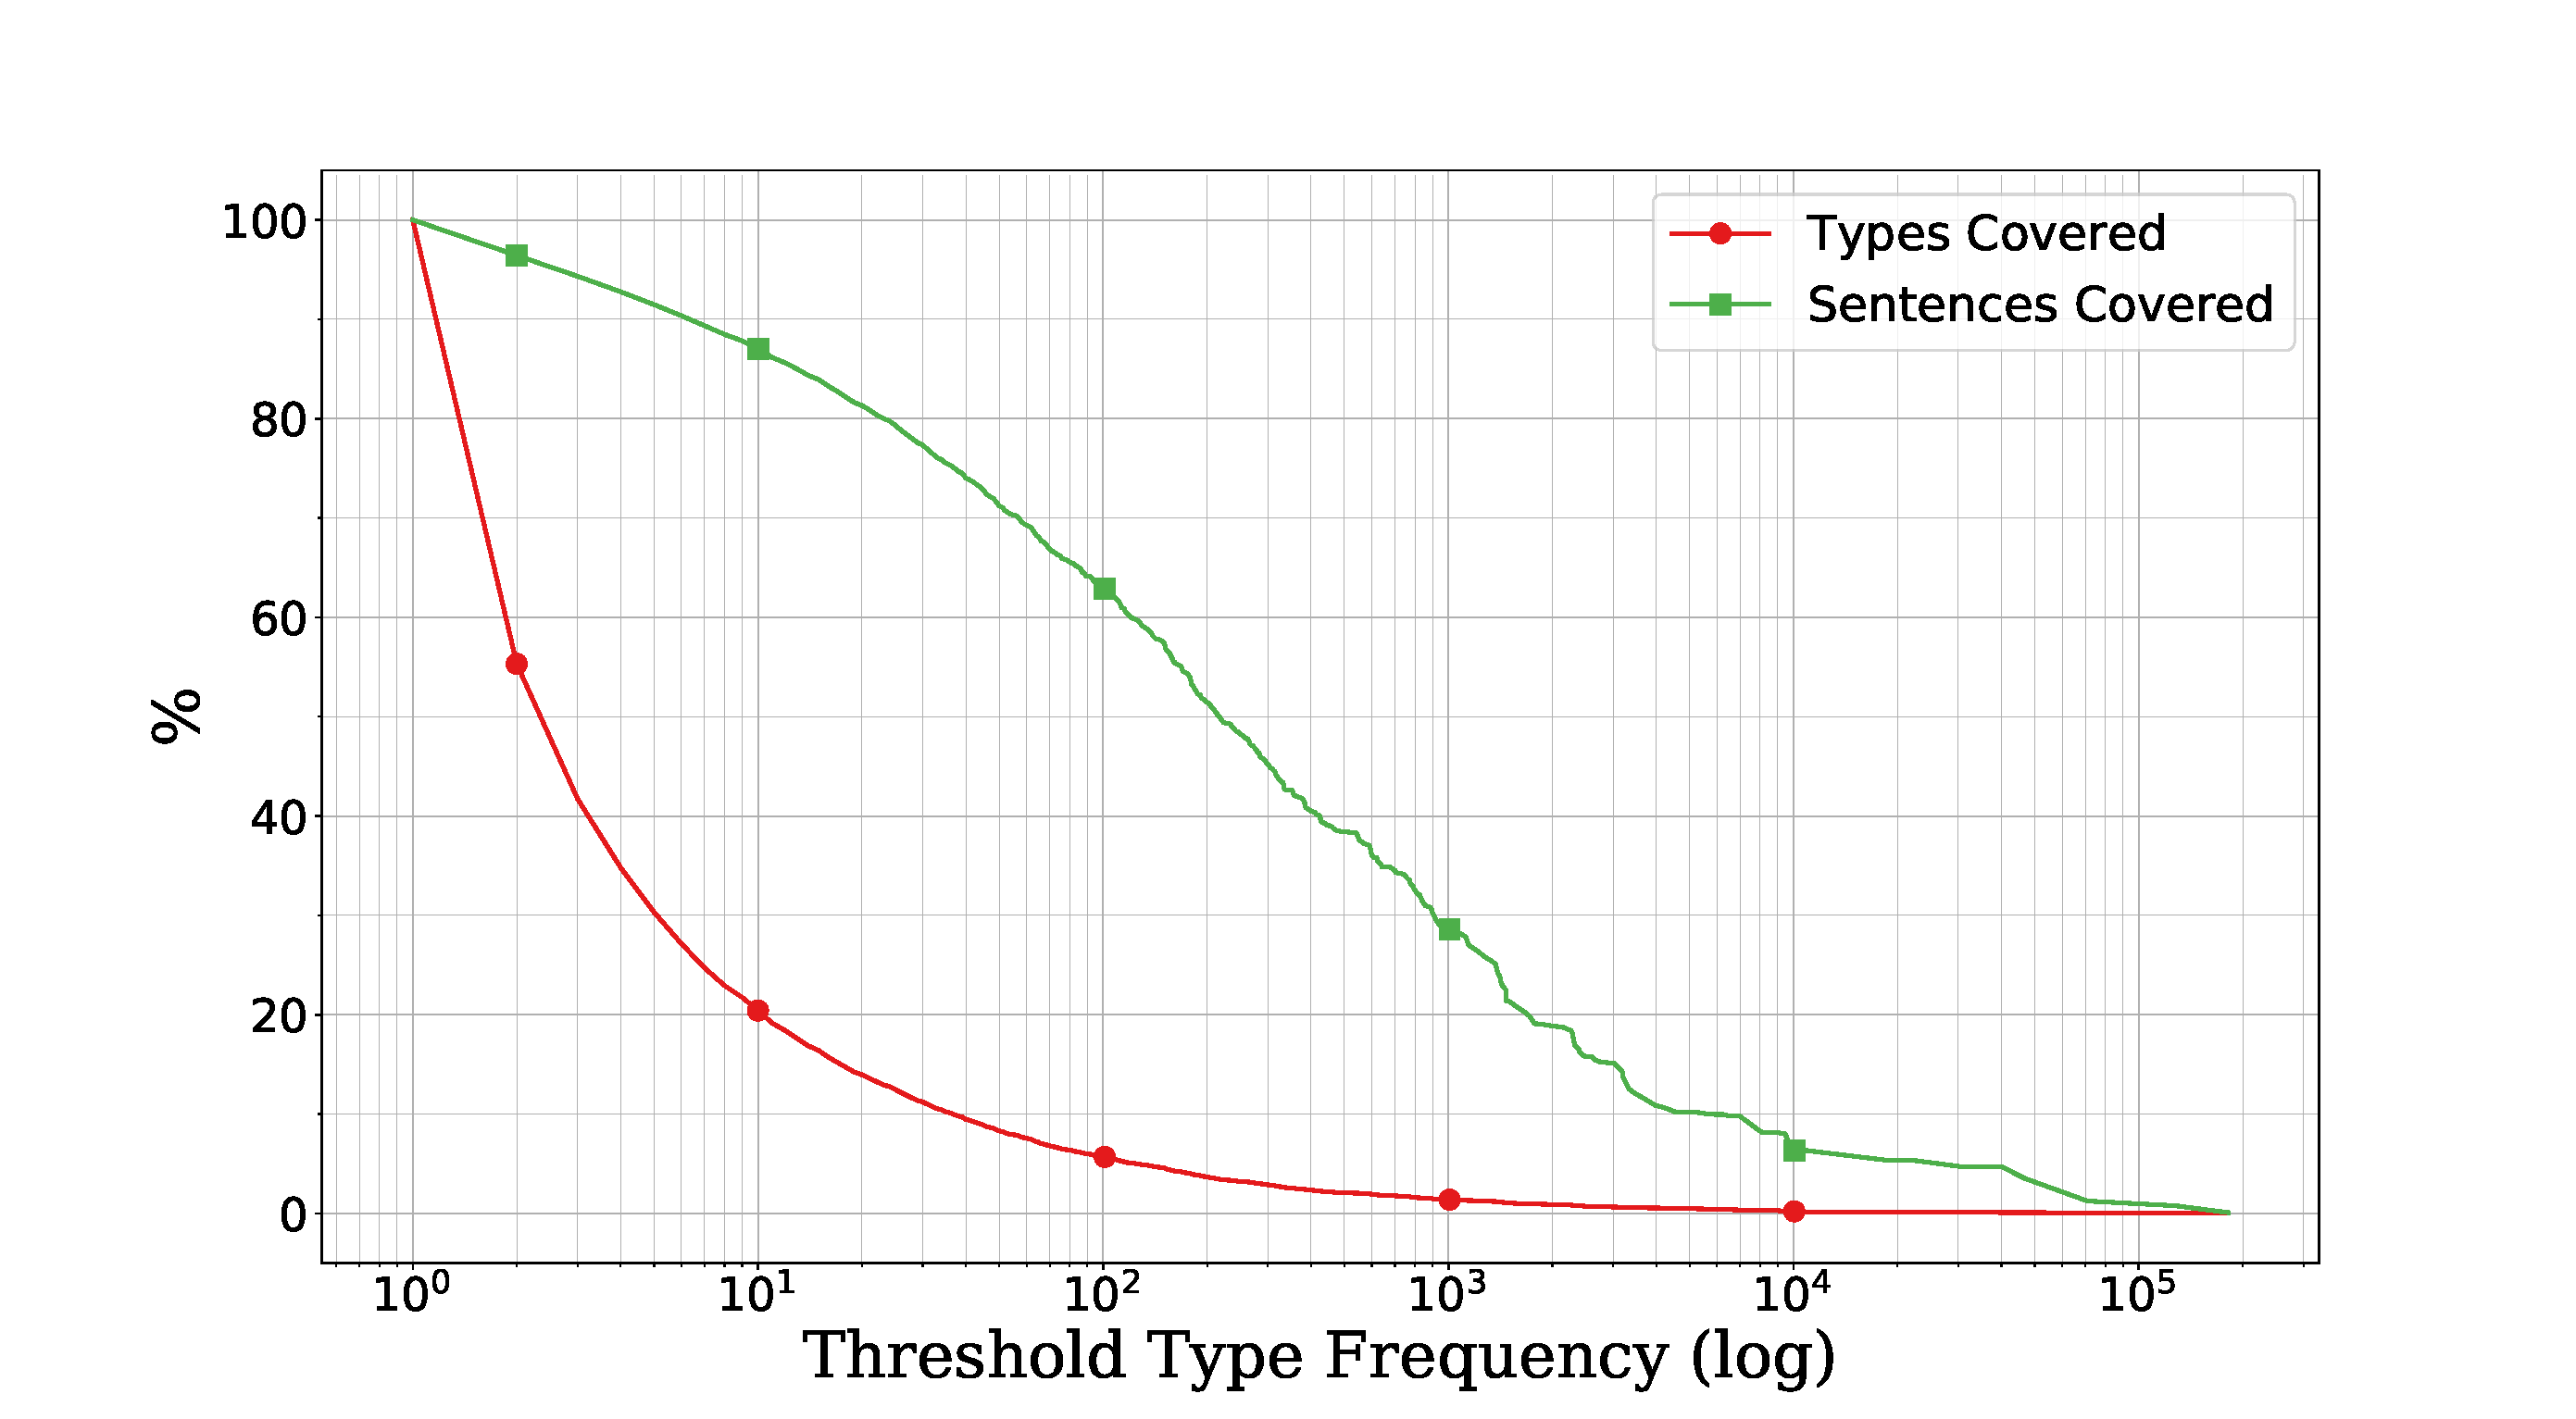
\includegraphics[scale=0.29]{Figures/sparsity.pdf}
    \caption[Extracted Type Sparsity]{Cumulative distribution of types and sentences covered as a function of type frequency. The horizontal axis depicts the logarithm of type occurrences in the corpus. The vertical axis depicts the percentage of types (red line)and sentences (green line) kept, if all types below an occurrence rate (or sentences containing them) are discarded.}
    \label{fig:type_sparsity}
\end{figure}

\section{Implementation}
Our setup imposes a number of design specifications that we must satisfy.
First, given the relatively free word order of the language, the type assignment process needs to be informed by the entirety of the input sentence.
In other words, our system must posses a global receptive field over the input.
Moreover, given the co-dependence between types, owing to their proof-theoretic properties, the output generation process has to be informed by prior outputs, i.e. the architecture needs to follow an auto-regressive formulation.
Finally, the presence of both short- and long-range dependencies, the first dictated by the type-forming grammar and the latter by the sentence-wide grammar, our system would benefit from representations that are global and sensitive to dynamic contexts, rather than local and iterative.

One recent proposal, originally intended for machine translation, perfectly fits the above requirements, namely the Transformer~\cite{vaswani2017attention}, which is an instance of a self-attention network.
To understand why that is the case and provide the necessary background for the rest of the subsection, we will begin by briefly going over the theoretical basis for self-attention networks and the mathematical formulation of the Transformer.

\subsection{Self-Attention}
Self-attention is a recently emerging idea that has gained traction in neural computation.
It is loosely inspired by cognitive attention, i.e. the ability to discriminate between sensory signals that are relevant to the current task and those that are not.
Neural attention was originally intended for use in image processing, but it has been adopted in the natural language processing domain as well, following its successful use in translation~\cite{bahdanau2014neural}.
Neural attention may be thought of as a means of content-based addressing, allowing a network to selectively shift its focus among arbitrary, non-contiguous indices over a set of dimensions of high-order tensors.
The general formulation requires a notion of similarity for the vector space occupied by some input and some context, as established by a matching function $s$:
\[
s: \mathbb{R}^d \otimes \mathbb{R}^d \to \mathbb{R}
\]
where $s(i, c)$  represents the real-valued weight of agreement between the input $i$ and the context $c$ (where $i, c \in \mathbb{R}^d$).
The output of this matching function may be used in a number of possible ways. 
To begin with, it allows the same vector $i$ to enact different roles under different scenarios, enabling context-sensitive processing.
Alternatively, $s(i,c)$ can exert a multiplicative factor over the value of $i$, deciding to what influence the latter will participate in further computation.
Attention then acts as a means of addressing that essentially allows highly precise information retrieval out of arbitrarily large tensors, superseding the need to lossily encode them in a fixed vector space.
Computationally, this is analogous to a program which refers only to variables invoked by its currently run instruction, where the variables are sought ought via partial or approximate reconstructions thereof using autoassociative memory.


If the function $s$ is continuous and differentiable, $s$ may be implemented as a neural function (fixed or parametric), through which gradients can flow during the backward pass, allowing either of its arguments to be optimized (soft attention).
Self-attention is a particular case of soft attention, in which the vectors of both $i$ and $c$ are not provided as direct arguments, but are in themselves productions of the network.
Crucially, the network is then tasked with finding the appropriate transformations such that its inner representations can be efficiently exploited by the matching function $s$.

\subsection{Transformers}
The first applications of attention involved the utilization of attentional interfaces on top of a recurrent network's hidden representations.
Transformers divert from that norm, instead modeling sequential processing purely via self-attention and position-local feed-forward connections.
This approach does away with the computational cost of recurrence (i.e. temporal iteration) and the conceptual constraints it imposes.
In finding an batch-efficient variation of attention, sequential processing may be done in a single step, owing to the lack of temporal dependencies.
For reasons of completeness, this section will briefly cover the main building blocks of a standard Transformer.

\paragraph{Scaled Dot-Product}
Given matrices $Q \in \mathbb{R}^{M\times d}$, $K, V \in \mathbb{R}^{N\times d}$, denoting queries, keys and values respectively, scaled dot-product attention $A$ is modeled as:
\[
A(Q,K,V) = \text{softmax}(\frac{QK^T}{\sqrt{d}})V
\]
The term $\frac{QK^T}{\sqrt{d}}$ is simply the dot-product of the queries against the keys scaled by the inverse of the square root of the vector space dimensionality.
It computes the weighted matching between $M$ queries and $N$ keys (both of dimensionality $d$), in the form of an $M$ by $N$ matrix.
The latter is normalized across its second dimension by application of the softmax function, thus converted into $M$ $N$-simplexes.
The result is matrix multiplied against $V$, producing a $M$ by $d$ matrix, each row of which is a weighted sum of the original rows of $V$.

\paragraph{Multi-Head Attention} A $k$-headed attention block is a neural function consisting of three sets of linear maps $f_{i,q}, f_{i, k}, f_{i, v}: \mathbb{R}^D \to \mathbb{R}^d$ and a linear map $f_o: \mathbb{R}^{kd} \to \mathbb{R}^D$.
It accepts three inputs $\hat{Q} \in \mathbb{R}^{M\times D}$ and $\hat{K}, \hat{V} \in \mathbb{R}^{N\times D}$ and produces an output $\text{MHA}(\hat{Q}, \hat{K}, \hat{V}) \in \mathbb{R}^{M \times D}$ as follows:
\[
\text{MHA}(\hat{Q}, \hat{K}, \hat{V}) = f_o \left ( 
    \text{concat} \left (
        \left [
            A \left (
                f_{i,q}(\hat{Q}),
                f_{i,k}(\hat{K}),
                f_{i,v}(\hat{V})
            \right )
        \
        \forall \ i \in 1,\dots, k
        \right ]
    \right )
\right )
\]
Practically, each $f_{i,x}$ is a parametric projection of its input to a lower-dimensional space.
The scaled dot-product of each of the $k$ projection triplets is computed, and they are concatenated together forming a matrix in $\mathbb{R}^{M\times kd}$.
The result is projected back into the original space by application of $f_o$.

\paragraph{Encoder Block} A transformer encoder block is a neural component that models the composition of a multi-headed attention block and a two-layer, position-local feed-forward network (FFN).
It receives as input a sequence of $M$ vectors, $X \in \mathbb{R}^{M\times D}$, to which it applies the multi-headed attention block producing an intermediate representation $H = \text{MHA}(X, X, X) \in \mathbb{R}^{M \times D}$.
The position-local network is then applied independently on each vector over the $M$ index of $H$.
Optionally, regularization in the form of layer normalization~\cite{lei2016layer} and dropout layers~\cite{hinton2012improving} as well as highway connections~\cite{srivastava2015highway} may be inserted before, between and/or after the encoder block's subcomponents.

\paragraph{Decoder Block} A transformer decoder block differs from the encoder block in two ways: it accepts two inputs $X \in \mathbb{R}^{M \times D}$ and $Y \in \mathbb{R}^{N\times D}$, and it contains two multi-head attention blocks.
The first computes the intra-attention of $Y$ over itself to produce a sequence of factored queries $Q_Y = \text{MHA}(Y, Y, Y)$.
The second computes the attention between the input $X$ and $Q_Y$: $H = \text{MHA}(Q_Y, X, X)$.
Finally, the position-wise transformation is applied on $H$ just as before.

\paragraph{Putting Things Together}
The overall architecture consists of an encoder and a decoder, each being a stack of their respective blocks.
The encoder is first applied over the full input sequence, producing contextually informed vectors over it.
The absence of recurrence necessitates the modulation of the input to distinguish between repetitions of the same item in a sequence; this is accomplished by adding a positional encoding over both input and output embeddings, implemented as a multi-dimensional sinusoidal wave.
The decoder then composes the decoder blocks as follows:
\begin{itemize}
    \item each block's $Y_i$ input is produced by the immediately prior block (where $Y_0$ is the vectorial representation of the output sequence produced up until the current timestep, right shifted once)
    \item each block's $X$ input is the encoder's output
    \item the output of the last decoder block is passed through a standard classifier to produce class labels over each output item
\end{itemize}

This flow ensures that the final output is informed by the full input sequence but also the preceding output sequence.
It is not bound to equal sequence lengths between input and output, and requires no lossy compression, unlike recurrent encoder/decoder architectures.
By masking the right-shifted output embeddings, the forward pass of the Transformer has minimal computational cost during training time, allowing faster training of deeper models.
During inference, temporal dependency is reintroduced by the need to operate on output embeddings which are not known in advance.
An abstract schematic view of the Transformer is given in Figure~\ref{fig:transformer}.

\begin{figure}
    \centering
    \begin{tikzpicture}[every text node part/.style={align=center},
                        every node/.style={transform shape},
                        scale=1,
                        miniblock/.style={
                            rectangle, 
                            inner sep=0pt,
                            rounded corners,
                            thick,
                            minimum width=50pt,
                            minimum height=25pt,
                            draw=gray!90},
                        encblock/.style={
                            rectangle, 
                            inner sep=0pt,
                            rounded corners,
                            very thick,
                            minimum width=70pt,
                            minimum height=100pt,
                            fill=gray!20,
                            draw=gray!90},
                        decblock/.style={
                            rectangle, 
                            inner sep=0pt,
                            rounded corners,
                            very thick,
                            minimum width=70pt,
                            minimum height=150pt,
                            fill=gray!20,
                            draw=gray!90},
                        textblock/.style={
                            rectangle,
                            inner sep=0pt,
                            outer sep=7.5pt,
                            minimum width=50pt,
                            minimum height=0pt},
                        dotblock/.style={
                            circle,
                            fill=black,
                            draw=black,
                            minimum size=3pt,
                            inner sep=0pt}
                        ]
        \definecolor{mha}{RGB}{253,184,99};
        \definecolor{ffn}{RGB}{178,171,210};
        \definecolor{linear}{RGB}{166,219,160};
        \definecolor{embedding}{RGB}{255,255,178};
        \node[textblock,align=left] (input) at (0, 0) {Input\\ Embeddings};
        
        \node[encblock] (enc1) at (0,3) {};
        \node[dotblock] (enc1prior) at (0,1.5) {};
        \node[miniblock, fill=mha] 
            (enc1mha) at (0,2.25) {MHA};
        \node[miniblock,fill=ffn] 
            (enc1ffn) at (0,3.75) {FFN};
            
        \node[encblock] (enc2) at (0,8) {};
        \node[dotblock] (enc2prior) at (0,6.5) {};
        \node[miniblock, fill=mha] 
            (enc2mha) at (0,7.25) {MHA};
        \node[miniblock,fill=ffn] 
            (enc2ffn) at (0,8.75) {FFN};
            
        \node[textblock] (enc_interm) at (0, 5.5) {\dots};

        \draw (input) edge[very thick,->] (enc1prior);
        \draw (enc1prior.center) edge[bend right, very thick] (enc1mha);
        \draw (enc1prior.center) edge[bend left, very thick] (enc1mha);
        \draw (enc1prior) edge[very thick] (enc1mha);
        \draw (enc1mha) edge[very thick,->] (enc1ffn);
        
        \draw (enc1ffn) edge[very thick] (enc_interm);
        \draw (enc_interm) edge[very thick,->] (enc2prior);
        \draw (enc2prior.center) edge[bend right, very thick] (enc2mha);
        \draw (enc2prior.center) edge[bend left, very thick] (enc2mha);
        \draw (enc2prior) edge[very thick] (enc2mha);
        \draw (enc2mha) edge[very thick,->] (enc2ffn);

        \node[textblock,align=left] (output) at (4, 0) {Output\\ Embeddings\\ (right-shifted)};
        
        \node[decblock] (dec1) at (4,3.8) {};
        \node[dotblock] (dec1prior) at (4,1.5) {};
        \node[miniblock, fill=mha] 
            (dec1mha) at (4,2.25) {MHA};
        \node[miniblock, fill=mha] 
            (dec1mmha) at (4,3.85) {MHA};
        \node[miniblock, fill=ffn] 
            (dec1ffn) at (4,5.6) {FFN};
        \node[dotblock] (dec1posterior) at (4, 3) {};
    
        \node[decblock] (dec2) at (4,10.8) {};
        \node[dotblock] (dec2prior) at (4,8.5) {};
        \node[miniblock, fill=mha] 
            (dec2mha) at (4,9.25) {MHA};
        \node[miniblock, fill=mha] 
            (dec2mmha) at (4,10.85) {MHA};
        \node[miniblock, fill=ffn] 
            (dec2ffn) at (4,12.6) {FFN};
        \node[dotblock] (dec2posterior) at (4, 10) {};
        
        \draw (output) edge[very thick,->] (dec1prior);
        \draw (dec1prior.center) edge[bend right, very thick] (dec1mha);
        \draw (dec1prior.center) edge[bend left, very thick] (dec1mha);
        \draw (dec1prior) edge[very thick] (dec1mha);
        \draw ($(dec1mha.north) + (-0.25, 0)$) edge[very thick,->] ($(dec1mmha.south) + (-0.25, 0)$);
        \draw (dec1posterior.center) edge[bend right, very thick] (dec1mmha);
        \draw (dec1posterior.center) edge[very thick] (dec1mmha);
        \draw (dec1mmha) edge[very thick,->] (dec1ffn);
        
        \node[textblock] (dec_interm) at (4, 7.3) {\dots};

        \node[miniblock, fill=linear] (classifier) at (8, 12.6) {Classifier};
        \draw (dec1ffn) edge[very thick,->] (dec_interm);
        \draw (dec_interm) edge[very thick] (dec2prior);
        \draw (dec2prior.center) edge[bend right, very thick] (dec2mha);
        \draw (dec2prior.center) edge[bend left, very thick] (dec2mha);
        \draw (dec2prior) edge[very thick] (dec2mha);
        \draw ($(dec2mha.north) + (-0.25, 0)$) edge[very thick,->] ($(dec2mmha.south) + (-0.25, 0)$);
        \draw (dec2posterior.center) edge[bend right, very thick] (dec2mmha);
        \draw (dec2posterior.center) edge[very thick] (dec2mmha);
        \draw (dec2mmha) edge[very thick,->] (dec2ffn);
        
        
        \node[textblock] (probabilities) at (8, 10.6) {Output Probabilities};
        \draw (classifier) edge[very thick,->] (probabilities);
        \draw   [decorate,
                very thick, 
                decoration={brace,amplitude=10pt}]
                (-1.5,1) -- (-1.5,10) node[black,midway,xshift=-1.3cm] 
{Encoder};
        \draw   [decorate,
                decoration={brace, amplitude=10pt,mirror},
                yshift=0pt,
                very thick]
                (5.5,1) -- (5.5,13.5) node[black,midway,xshift=1.3cm] {Decoder};
        \draw (dec2ffn) edge[very thick,->] (classifier);
        
        \draw [rounded corners=5pt, very thick,->] (enc2ffn)--(0,10)--(dec2posterior);
        \draw [rounded corners=5pt, very thick,->] (2,10)--(2,3)--(dec1posterior);
        \node[inner sep=0] at (2, 10) {};
        
        \node[miniblock, align=left, fill=embedding] (emb) at (8,0) {\small Embedding \\ Layer};
        \draw (probabilities) edge[->, dotted, very thick] node[right] {$argmax$} (emb);
        \draw (emb) edge[->, dotted, very thick] (output);

    \end{tikzpicture}
    \caption[Transformer Architecture]{Abstract view of the Transformer architecture, with unspecified number of Encoder and Decoder layers. During training, the output embeddings are precomputed. During inference, the embedding of the most probable output class of each timestep is iteratively computed and appended to the previous output embeddings, as depicted by the dotted line.}
    \label{fig:transformer}
\end{figure}

\subsection{Model}
The supertagging model's architecture follows the standard encoder-decoder paradigm commonly employed by sequence-to-sequence models. 
It accepts a sequence of words as input, and produces a longer sequence of atomic symbols as output.
A high-level overview, together with an example input/output pair, are presented in Figure~\ref{fig:modelandio}.
The source code for our model is publicly available and can be found at \url{https://github.com/konstantinosKokos/Lassy-TLG-Supertagging}.
The custom implementation of the Transformer used by the model can be found at \url{https://github.com/konstantinosKokos/UniversalTransformer}.

\begin{figure}
\centering
\begin{subfigure}[b]{1\textwidth}
\begin{tikzpicture}[every text node part/.style={align=center},
 every node/.style={transform shape},
 scale=0.6,
block/.style={rectangle, inner sep=0pt, minimum width=120pt, minimum height=60pt, rounded corners, ultra thick},
str/.style={rectangle, inner sep=0pt, minimum width=120pt, minimum height=20pt},
arrow/.style={->, ultra thick},
pwise/.style={circle, inner sep=0pt, minimum size=10pt},
smallblock/.style={circle, inner sep=5pt, minimum size=12pt, rounded corners, thick}]

	\node[str] (sentence) at (0, 5) {Input Sentence};		
	\node[str] (symbols) at (7.5, 5) {Output Sequence};

    \definecolor{first}{RGB}{82,82,82}
    \definecolor{enc}{RGB}{253,192,134}
    \definecolor{dec}{RGB}{127,201,127}
    \definecolor{dec2}{RGB}{140,220,140}
    \definecolor{emb}{RGB}{190,174,212}

	\node[block, draw=black, fill=gray!10, draw=gray!130] (elmo) at (0,8) {\textcolor{gray!110}{ELMo}};
	\node[block, draw=black, fill=enc] (te) at (0,12) {\textbf{Encoder}};
	\node[block, draw=black, fill=emb] (se) at (7.5,8) {\textbf{Embedding}};
	\node[block, draw=black, fill=dec2] (td2) at (7.75, 12.25) {};
	\node[block, draw=black, fill=dec] (td) at (7.5,12) {\textbf{Decoder}};
	\node[block, draw=black, fill=emb] (set) at (15,12) {\textbf{Embedding}\\ (transposed)};	
	\node[smallblock, draw=black] (ss) at (15, 8) {$\sigma$};
	\node[smallblock, draw=black] (am) at (12, 8) {$\alpha$};
	\node[str] (out) at (15,5) {Output Probabilities};	
	

	\draw (symbols) edge [arrow, gray!130] node[right] {M symbols} (se);
	\draw  (sentence) edge [arrow, gray!130] node[left] {N words} (elmo);
	\draw  (elmo) edge [arrow, gray!130] node[left] {Sentence Embedding\\ $\mathbb{R} ^ {N \times 1024}$} (te);
	\draw  (se) edge [arrow] node[right] {Symbol Embeddings\\ $\mathbb{R} ^ {M \times 1024}$} (td);
	\draw ($(te.east) + (0, 0.5)$) edge [arrow] node[above] {Encoder Keys\\ $\mathbb{R}^ {N \times 1024}$} ($(td.west) + (0, 0.5)$);
	\draw ($(te.east) + (0, -0.5)$) edge [arrow] node[below] {Encoder Values\\ $\mathbb{R}^ {N \times 1024}$} ($(td.west) + (0, -0.5)$);\
	\draw ($(td.east) + (0.25, 0)$) edge [arrow] node[above] {Decoder Values\\ $\mathbb{R}^ {M \times 1024}$} (set);
	\draw (set) edge [arrow] node[right] {Class Weights} (ss);
	\draw (ss) edge [arrow] (out);
	\draw (set.south) [dotted, very thick] .. controls +(-1,0) and +(-0.5, 0.5) .. (am.north);
	\draw (am.south) [dotted, very thick, ->] .. controls +(0,-0.5) and +(2, ) .. (symbols.east);
\end{tikzpicture}
\caption{The model architecture, where $\sigma$ and $\alpha$ denote the \textit{sigsoftmax} and \textit{argmax} functions respectively, grayed out components indicate non-trainable components and the dotted line depicts the information flow during inference.}
\label{fig:model}
\end{subfigure}
\vspace{10pt}
\begin{subfigure}[b]{1\textwidth}
\begin{minipage}{1\textwidth}
\gll {is (\textit{is})} \quad {er (\textit{there})} \quad {een (\textit{a})} \quad {toepassing (\textit{use})} \quad {voor (\textit{for})} \quad {lineaire (\textit{linear})} \quad {logica (\textit{logic})}\\
$\textsc{np}\myrightarrow{su}\textsc{s}_\text{main}$
\quad
$\textsc{s}_\text{main}\myrightarrow{mod}\textsc{s}_\text{main}$
\quad
\small $\textsc{np}\myrightarrow{det}\textsc{np}$
\quad
\small $\textsc{np}$
\quad
\small $\textsc{np}\myrightarrow{obj1}\textsc{np}\myrightarrow{mod}\textsc{np}$
\quad
\small $\textsc{np}\myrightarrow{mod}\textsc{np}$
\quad
\small $\textsc{np}$\\
\trans $\myrightarrow{su},\textsc{np}, \textsc{s}_\text{main}, \text{\#}, \myrightarrow{mod},\textsc{s}_\text{main}, \textsc{s}_\text{main}, \text{\#},\myrightarrow{det},\textsc{np}, \textsc{np}, \text{\#},\textsc{np},\myrightarrow{obj1},\textsc{np}, \myrightarrow{mod},\textsc{np}, \textsc{np}, \text{\#}\myrightarrow{mod},\textsc{np}, \textsc{np}, \text{\#},\textsc{np},\text{\#}$
\end{minipage}
\caption{Input-output example pair for the sentence ``is er een toepassing voor lineaire logica?'' (\textit{is there a use for linear logic?}). The first two lines present the input sentence and the types that need to be assigned to each word. The third line presents the desired output sequence, with types decomposed to atomic symbol sequences under polish notation, and \# used as a type separator.}
\label{fig:io}
\end{subfigure}
\caption[Supertagging Architecture and I/O Pair]{Supertagging Architecture~(\ref{fig:model}) and an example input-output pair~(\ref{fig:io}).}
\label{fig:modelandio}
\end{figure}

\paragraph{Language Model Pretraining}
Empirical evidence~\cite{D17-1039} suggests that sequence-to-sequence architectures benefit from unsupervised pretraining of their encoder and decoder components as independent language models.
Language models are statistical models that estimate the probability distribution of sequences (e.g. sentences).
They can be used to either rank the probability of a whole sequence, or as generators, for instance predicting a sequence's continuation given a variable-length prefix thereof, by taking the maximum-likelihood estimate of the conditional distribution $
p(w_t | w_{0},\dots,w_{t-1})
$.

Adhering to this, we incorporate a pretrained Dutch ELMo into our encoder~\cite{dutch_elmo}.
ELMo was originally proposed as an architecture for producing deep contextualized word representations~\cite{peters2018deep}, where deep is reference to the use of a stacked, bi-directional LSTM to process the input sequence. 
A weighted combination of the representations of each layer is then utilized as input by downstream task-specific models, where the weighting terms are functions to be learned by the task models.
The variation we are using was trained as a task-agnostic language model on large-scale corpora, and the 1024-dimensional representations it constructs were proven highly adequate for parsing tasks.
The choice of ELMo's output as our sentence-level input carries relays the added strength of utilizing subword-level information; a character-level LSTM participates in the construction of ELMo's lowest-level (context-independent) token representations.

Constructing a decoder-side language model is less of a straightforward decision.
The size of Lassy-Small prohibits pretraining, as this would require splitting into two disjoint subsets (thus reducing the amount of data available to the end-to-end supertagger); this necessitates the use of a different corpus.
Our extraction algorithm is applicable to the silver-standard Lassy-Large, the size of which is certainly appealing for such an endeavour.
However, the quality of its annotations is lacking, reducing the potential benefits from pretraining.
Further, its larger size, in conjunction with the more irregular types (a by-product of the frequency of erroneous annotations) would be a confounding factor in evaluating our model's ability to construct new types.
Considering the above, we refrain from pretraining the decoder in the current setting.

\paragraph{Transformer} Even though ELMo acts as an encoder already, its representations are not necessarily optimal to use as is.
Adapting its representations to the domain is a costly process; ELMo counts a very large number of parameters, making it prone to overfit our dataset.
Instead, we treat it as a static function and process its output with a single-layer Transformer encoder of 3 attention heads.
In practice, since ELMo's parameters are hard-set and not affected by the backward pass, we may precompute the embeddings of our sentences in advance and feed those onto the rest of the network.

The decoding process is accomplished by 2-layer Transformer decoder. 
As the decoder needs to cast its predictions from a broader range of contexts, due to it processing information at a higher granularity scale, we increase its number of attention heads to 8.

We follow the original Transformer formulation in all but one point; we model the position-wise feed-forward transformation that is internal to the encoder and decoder layers as a two-layer, dimensionality preserving network.
We replace the linear rectifier of the intermediate layer with the empirically superior and statistically grounded Gaussian Error Linear Unit~\cite{gelu}:
\[
\text{GELU}(x) = 0.5x 
\left ( 
    1+\text{tanh}
        \left (
            \sqrt{2/\pi}
                \left (
                    x+0.044715x^3
                \right )
        \right )
\right )
\]

Overall, the network is tasked with modeling the probability distribution of the next atomic symbol at timestep $t$, $a_t$, conditional on all previous predictions $a_0,\dots,a_{t-1}$ and the full input sequence $w_0,\dots,w_\tau$, as parameterized by its trainable weights $\theta$:
\[
p_\theta(a_t|a_0,\dots,a_{t-1},w_0,\dots,w_\tau)
\]


\paragraph{Embedding} Since there are no pretrained embeddings for the output tokens, we train an atomic symbol embedding layer alongside the rest of the network.
The Transformer's formulation gives us no say on the dimensionality of the output space, as it has to match that of the input--- 1024.
This is not optimal, as the number of unique output tokens is one order of magnitude lower than the dimensionality, making the scale of the representations redundant.
To recover from this and make further use of the extra parameters, we use the transpose of the embedding matrix as our output classifier. 
Concretely, the embedding matrix is a linear map from $\mathbb{R}^{|\mathcal{A}|}$ to $\mathbb{R}^{1024}$, where $\mathcal{A}$ the set of atomic symbols used by the supertagger.
Hence, it's transpose is a linear map from $\mathbb{R}^{1024}$ to $\mathbb{R}^{|\mathcal{A}|}$, which may be reused to convert the transformer's 1024-dimensional output back into class weights.
These weights are converted into probabilities in the $|\mathcal{A}|$-simplex by application of the sig-softmax function~\cite{kanai2018sigsoftmax}, a softmax variant that enjoys stronger statistical approximation properties:
\[
\text{sigsoftmax}(x_i) = \frac{e^{x_i}\sigma(x_i)}{\sum_j{e^{x_j}\sigma(x_j)}}
\]

\subsection{Digram Encoding}
Predicting type sequences one atomic symbol or connective at a time provides the vocabulary to construct new types, but results in elongated target output sequence lengths. Note that if lexical categories are, on average, made out of $c$ atomic symbols, the overall output length is a constant factor of the sentence length, i.e. there is no change of complexity class with respect to a traditional supertagger.
As a countermeasure, we experiment with {\it digram encoding}, creating new atomic symbols by iteratively applying pairwise merges of  the most frequent intra-type symbol digrams~\cite{bpe}, a practice already shown to improve generalization for translation~\cite{bpe2} and language modeling tasks~\cite{gpt}. 
To evaluate performance, we revert the merges back into their atoms after obtaining the predictions.

With no merges, the model has to construct types and type sequences using only atomic types and connectives.
As more merges are applied, the model gains access to extra short-hands for subsequences within longer types, reducing the target output length, and thus the number of interactions it has to capture.
This, however, comes at the cost of a reduced number of full-type constructions effectively seen during training, while also increasing the number of implicit rules of the type-forming context-free grammar.
If merging is performed to exhaustion, all types are compressed into single symbols corresponding to the indivisible lexical types present in the treebank. 
The model then reduces to a traditional supertagger, never having been exposed to the internal type syntax, and loses the potential to generate new types.

\subsection{Experiments}
\paragraph{Training}
In all described experiments, the model is run on the subset of sample sentences that are at most 20 words long. 
We use a train/val/test split of 80/10/10; it is worth pointing out that the training set contains only $\sim$85\% of the overall unique types, the remainder being present only in the validation and/or test sets.
Training takes place with a batch size of 128, and sentences are padded to the maximum in-batch length. 
Training to convergence takes, on average, eight hours \& 300 epochs for the training set of 45000 sentences on a GTX1080Ti. 
Results are averaged over 5 repetitions.

Accuracy is reported on the type-level; that is, during evaluation, we predict atomic symbol sequences, then collapse subtype sequences into full types and compare the result against the ground truth. 
Notably, a single mistake within a type is counted as a completely wrong type. 

For the training algorithm, we adopt the training scheme originally proposed by Vaswani et al~\cite{vaswani2017attention}, which is unique in two ways.
First, rather than using standard cross-entropy as the objective function, it instead optimizes Kullback-Leibler divergence, a measure of distance between probability distribution.
The distributions compared are the network's predictions and an artificial distribution of the ground truth.
The latter is constructed by subtracting a fixed percentage of the probability mass from the true label, which is then uniformly spread across the remaining labels.
This practically forces the network to be less certain of its predictions, increasing its generalization capacity.
Moreover, it utilizes an adaptive learning rate, linearly increasing over a number of training iterations, then exponentially decaying until termination.
We set the amount of redistributed probability mass to 20\%, double that of the original proposal; a change that is crucial in order to discourage the network from memoizing common type patterns.
We apply dropout in between all network connections, at a rate of 20\%.

\paragraph{Results}
Our experiments involve a fully constructive model employing no merges ($\text{M}_0$), a fully merged one i.e. a traditional supertagger, ($\text{M}_\infty$), and three in-between models trained with 50, 100 and 200 merges ($\text{M}_{50}$, $\text{M}_{100}$ and $\text{M}_{200}$ respectively).
Table~\ref{table:numbers} displays the models' accuracy. 
In addition to the overall accuracy, accuracy over different bins of type frequencies is displayed, as measured in the training data: unseen, rare (1-10), medium (10-100) and high-frequency ($>$ 100) types.

\begin{table}
\centering
\newcommand{\ra}[1]{\renewcommand{\arraystretch}{#1}}
\ra{1.1}
\hspace{-10pt}
\begin{tabularx}{0.49\textwidth}{@{}Xsssss@{}}
{} &  \multicolumn{5}{c}{\centering Type Accuracy}\\
\cmidrule{2-6}
\multicolumn{1}{l}{}  &  \small Overall & \small Unseen & \small  Freq & \small Freq & \small Freq \\
\multicolumn{1}{l}{Model}  &  {} & \small Types & \small  1-10 & \small 10-100 & \small $>$100 \\
\cmidrule[0.001em]{1-6}
\centering $\text{M}_{0}$  & \textbf{ 88.05} & \textbf{19.2} & \textbf{45.68} & \textbf{65.62} & 89.93\\
\cmidrule[0.001em]{1-6}
\centering $\text{M}_{50}$  & 88.03 & 15.97 & 43.69 & 64.33 & \textbf{90.01}\\
\centering $\text{M}_{100}$ & 87.87 & 15.02 & 41.61 & 63.71 & 89.9 \\
\centering $\text{M}_{200}$ & 87.54 & 11.7 & 39.56 & 62.4 & 89.64\\
\cmidrule[0.001em]{1-6}
\centering $\text{M}_{\infty}$ & 87.2 & - & 23.91 & 59.03 & 89.89\\
\end{tabularx}
\caption[Supertagger Performance]{Model performance at different merge scales, with respect to training set type frequencies. $\text{M}_i$ denotes the model at $i$ merges, where $\text{M}_\infty$ means the fully merged model. For the fully merged model there is a 1 to 1 correspondence between input words and output types, so we do away with the separation symbol.}
\label{table:numbers}
\end{table}

Table~\ref{table:numbers} shows that all constructive models perform overall better than $\text{M}_{\infty}$, owing to a consistent increase in their accuracy over unseen, rare, and mid-frequency types.
This suggests significant benefits to using a representation that is aware of the type syntax.
Additionally, the gains are greater the more transparent the view of the type syntax is, i.e. the fewer the merges.
The merge-free model $\text{M}_0$ outperforms all other constructive models across all but the most frequent type bins, reaching an overall accuracy of 88.05\% and an unseen category accuracy of 19.2\%.

What is also interesting to examine is the models' ``imaginative'' precision, i.e.,  how often do they generate new types to analyze a given input sentence, and, when they do, how often are they right (Table~\ref{table:imagination}). 
Although all constructive models are eager to produce types never seen during training, they do so to a reasonable extent. 
Similar to their accuracy, an upwards trend is also seen in their precision, with $\text{M}_0$ getting the largest percentage of generated types correct. 

Together, the results indicate that the type-syntax is not only learnable, but also a representational resource that can be utilized to tangibly improve a supertagger's generalization and overall performance.

\begin{table}
\centering
\noindent
\newcommand{\ra}[1]{\renewcommand{\arraystretch}{#1}}
\ra{1.1}
\begin{tabularx}{0.49\textwidth}{@{}Xsss@{}}
\multicolumn{1}{l}{Model}  &  New Types & Unique & Correct \small (\%)\\
\multicolumn{1}{l}{}  &  Generated  &  &  \\
\cmidrule[0.01em]{1-4}
\centering $\text{M}_{0}$  & 213.6 & 199.2 &  \textbf{44.39} \small (\textbf{20.88}) \\
\centering $\text{M}_{50}$  & 186.6 & 174.2 & 37.89 \small (20.3) \\
\centering $\text{M}_{100}$  & 187.8 & 173.4 & 34.31 \small (18.27) \\
\centering $\text{M}_{200}$  & 190.4 & 178.8 & 27.46 \small (14.42) \\
\end{tabularx}
\caption[Supertagger Unseen Type Precision]{Repetition-averaged unseen type generation and precision.}
\label{table:imagination}
\end{table}

\paragraph{Baselines}
In order to evaluate our model's performance in comparison to established supertagging practices, we experimented with RNN-based encoder-decoder architectures. 
We tried training a single-layer BiGRU encoder over the ELMo representations, connected to a single-layer GRU decoder, following~\cite{gru}; the model took significantly longer to train and yielded far poorer results.
We hypothesize that the encoder's fixed length representation is unable to efficiently capture all of the information required for decoding a full sequence of atomic symbols, inhibiting learning.

As an alternative, we tried a separable LSTM decoder operating individually on the encoder's representations of each word. 
Even though this model was faster to train and performed marginally better compared to the previous attempt, it still showed no capacity for generalization over rare types. 
This is unsurprising, as this approach assumes that the decoding task can be decomposed at the type-level; crucially, the separable decoder's prediction over a word cannot be informed by its predictions spanning other words, an information flow that evidently facilitates learning and generalization.

\subsection{Analysis}
\paragraph{Type Syntax}
To assess the models' acquired grasp of the type syntax, we inspect type predictions in isolation.
Across all merge scales and consistently over all trained models, all produced types (including unseen ones) are \textit{well-formed}, i.e. they are indeed words of the type-forming grammar.
Further, the types constructed perfectly follow along our implicit notational conventions such as the obliqueness hierarchy.

Even more interestingly, for models trained on non-zero merges it is often the case that a type is put together using the correct atomic elements that together constitute a merged symbol, rather than the merged shorthand trained on.
Judging from the above, it is apparent that the model gains a functionally complete understanding of the type-forming grammar's syntax, i.e. the means through which atomic symbols interact to produce types.

\paragraph{Sentence Syntax}
\begin{figure}
\centering
\begin{minipage}{1\textwidth}

\gll {in (\textit{to})}  {hoeverre (\textit{what-degree})} \quad {zal (\textit{will})} \quad {het (\textit{the})} \quad {rapport (\textit{report})} \quad {dan (\textit{then})} \quad {nog (\textit{still})} \quad {een (\textit{a})} \quad {rol (\textit{role})} \quad {spelen (\textit{play})}\\ $\textsc{\textbf{bw}}\myrightarrow{\textbf{obj1}}\textbf{((}\textsc{\textbf{inf}}\myrightarrow{\textbf{mod}}\textsc{\textbf{inf}}\textbf{)}\rightarrow\textsc{\textbf{sv1}}\textbf{)}\myrightarrow{\textbf{body}}\textsc{\textbf{whq}}$
\quad 
\small $\textsc{bw}$
\quad
\small $\textsc{inf}\myrightarrow{vc}\textsc{np}\myrightarrow{su}\textsc{sv1}$
\quad
\small $\textsc{n}\myrightarrow{det}\textsc{np}$
\quad
\small $\textsc{n}$
\quad
\small $\textsc{inf}\myrightarrow{mod}\textsc{inf}$
\quad
\small $\textsc{inf}\myrightarrow{mod}\textsc{inf}$
\quad
\small $\textsc{n}\myrightarrow{det}\textsc{np}$
\quad
\small $\textsc{n}$
\quad
\small $\textsc{np}\myrightarrow{obj1}\textsc{inf}$\\
\end{minipage}
\caption[Unseen Type Example]{Type assignments for the correctly analyzed wh-question ``in hoeverre zal het rapport dan nog een rol spelen'' (\textit{to what extent will the report still play a role}) involving a particular instance of \textit{pied-piping}. The type of ``in'' was never seen during training; it consumes an adverb as its prepositional object, to then provide a third-order type that turns a verb-initial clause with a missing infinitive modifier into a wh-question. Such constructions are a common source of errors for supertaggers, as different instantiations require unique category assignments.}
\label{fig:electricity}
\end{figure}

Beyond the spectrum of single types, we examine type assignments in context.

We first note a surprising ability to correctly analyze syntactically complex constructions requiring higher-order reasoning, even in the presence of unseen types.
An example of such an analysis is shown in Fig~\ref{fig:electricity}.

For erroneous analyses, we observe a strong tendency towards self-consistency.
In cases where a type construction is wrong, types that interact with that type (as either arguments or functors) tend to also follow along with the mistake.
On one hand, this cascading behavior has the effect of increasing error rates as soon as a single error has been made.
On the other hand, however, this is a sign of an implicitly acquired notion of phrase-wide well-typedness, and exemplifies the learned long-range interdependencies between types through the decoder's auto-regressive formulation.
On a related note, we recognize the most frequent error type as misconstruction of conjunction schemes. 
This was, to a degree, expected, as coordinators display an extreme level of lexical ambiguity, owing to our extracted grammar's massive type vocabulary. 

\paragraph{Output Embeddings}
Finally, we draw  attention to a thus far ignored aspect of the architecture. 
Our network trains not only the encoder-decoder stacks, but also an embedding layer of atomic symbols.
We can extract this layer's outputs to generate vectorial representations of atomic types and binary connectives, which essentially are high-dimensional character-level embeddings of the type language.
Figure~\ref{fig:symbol_tsne} displays a 2-dimensional tSNE~\cite{maaten2008visualizing} reconstruction of the embedding space, where some degree of structure is immediately apparent.
Considering that dense supertag representations have been shown to benefit parsing~\cite{kasai-etal-2017-tag}, our atomic symbol embeddings may be further utilized by downstream tasks, as a highly refined source of type-level information.

\begin{figure}[t]
    \centering
    \hspace{-70pt}
    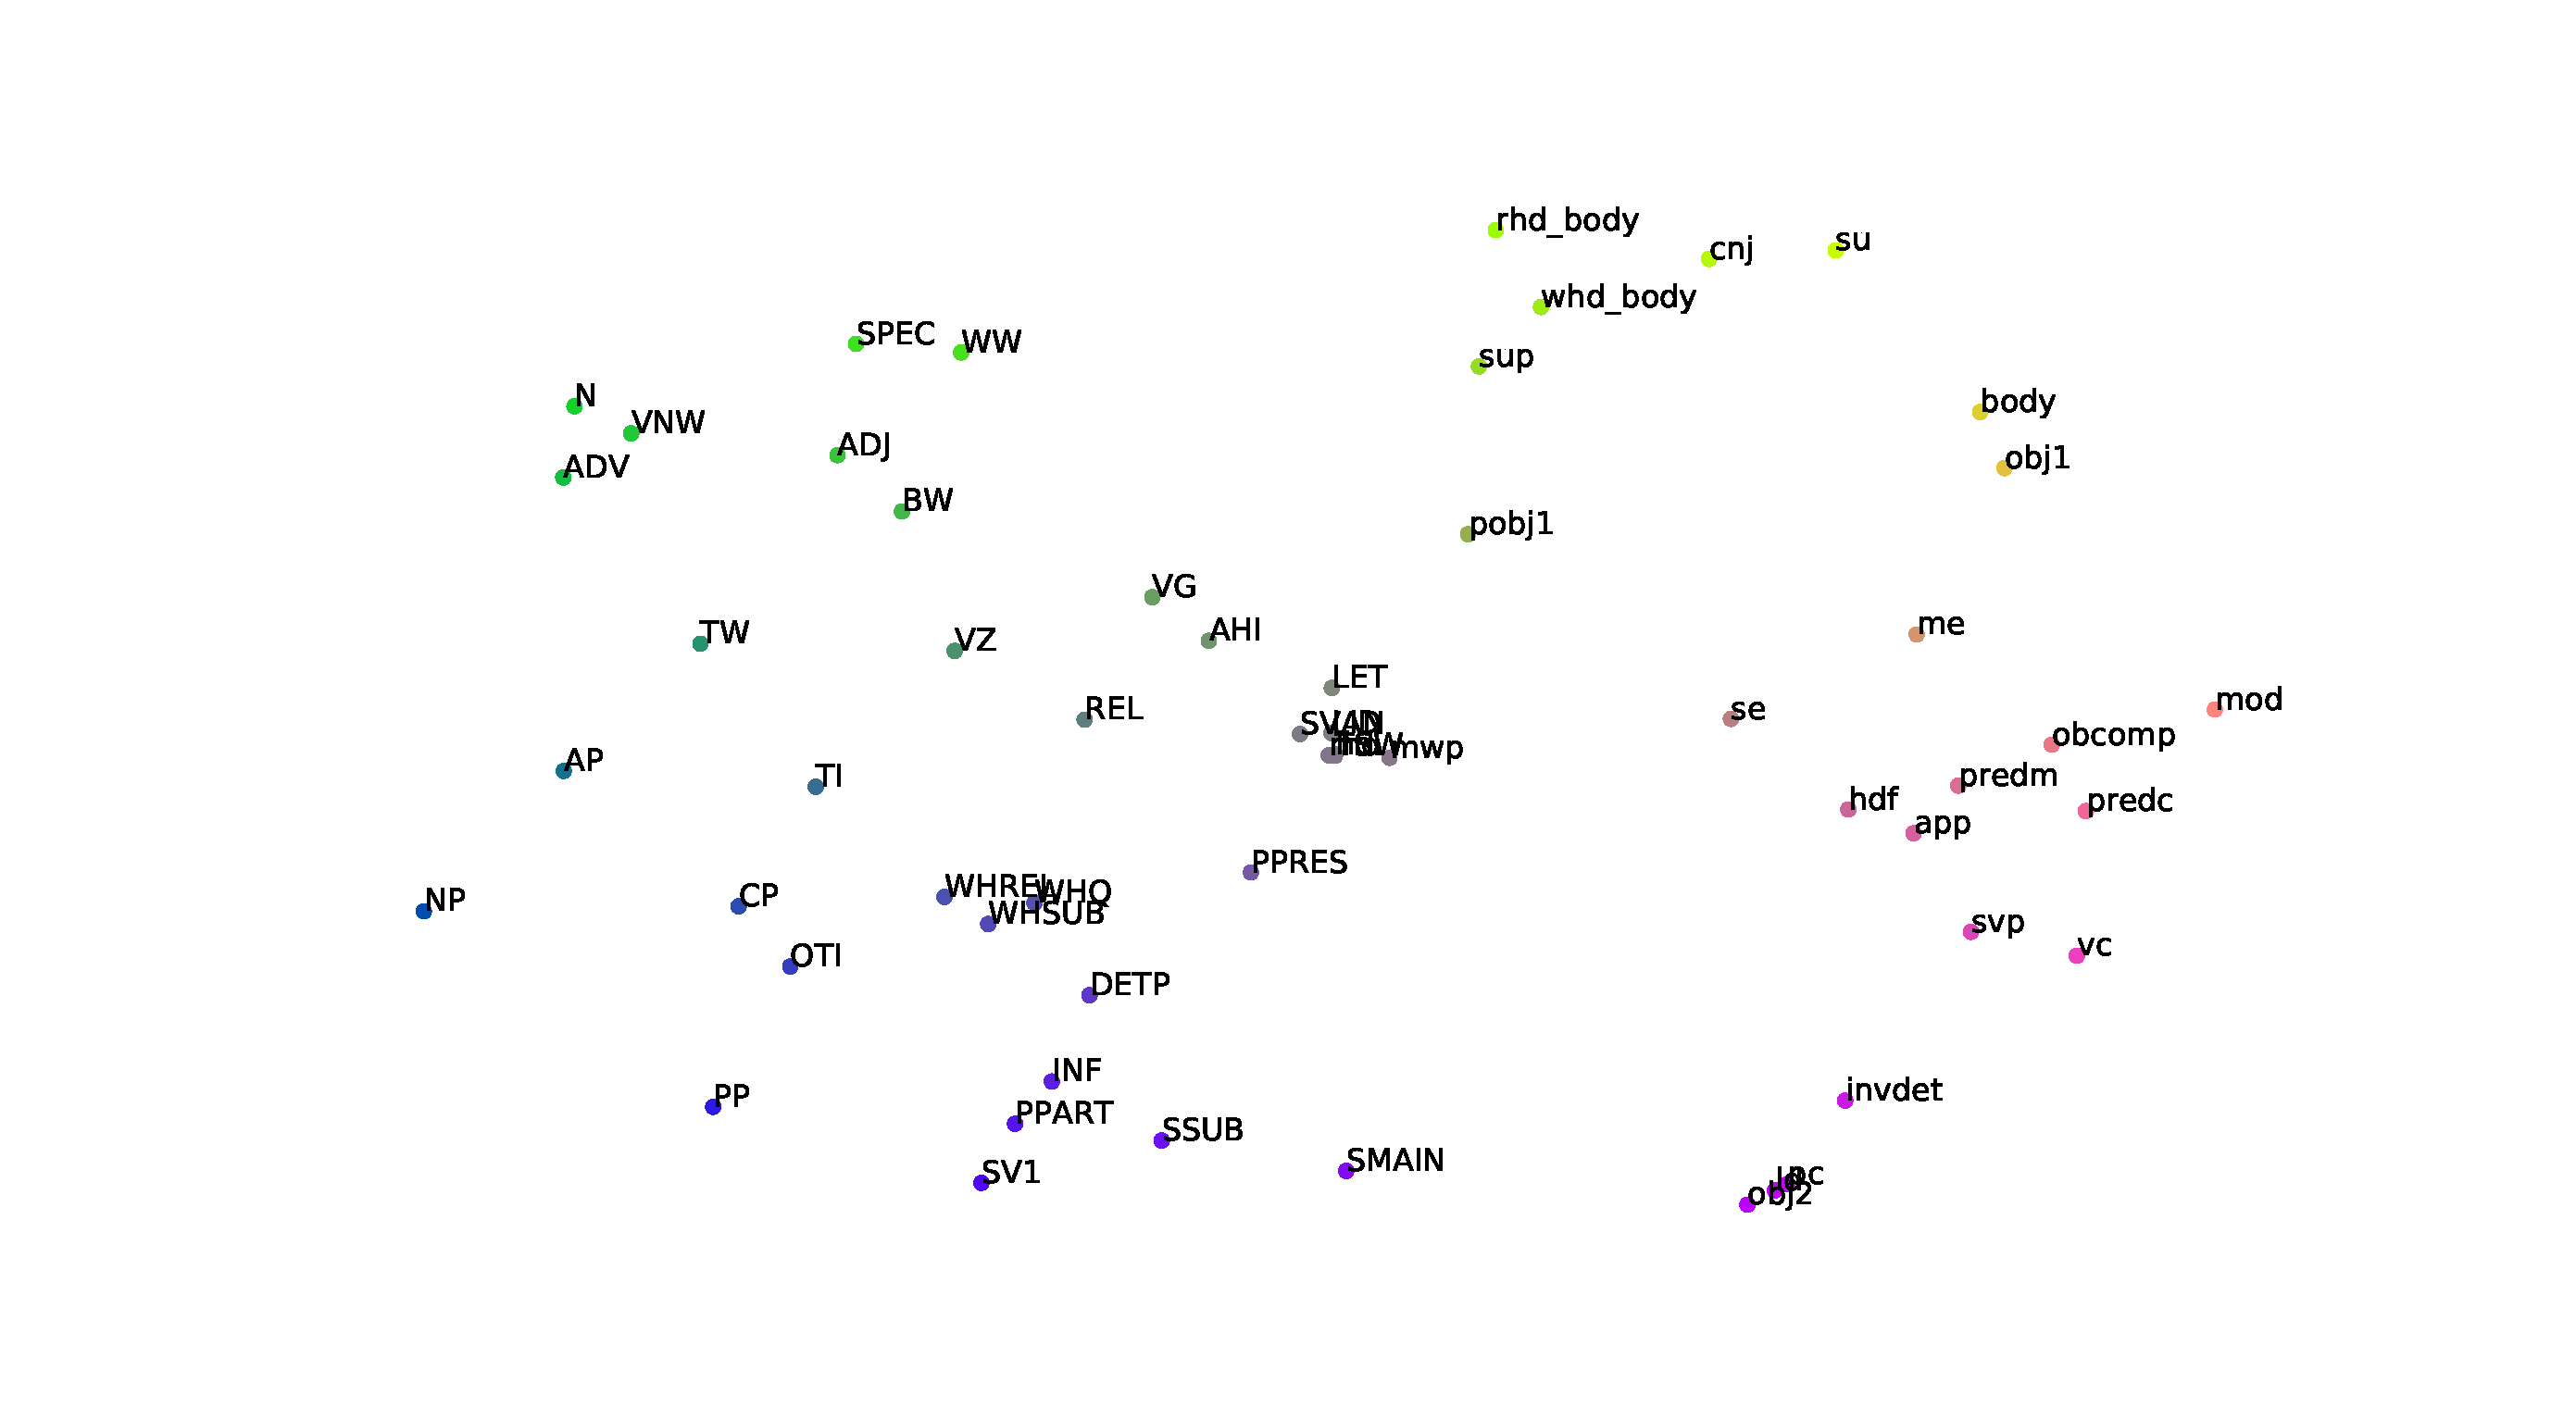
\includegraphics[scale=0.29]{Figures/cluster.pdf}
    \caption[tSNE of Atomic Symbol Embeddings]{2-d tSNE projection of the embedding space. Two major clusters are formed by binary connectives (lowercase, east) and atomic types (uppercase, west). Smaller clusters are also noticeable between sentential types, indirect verb arguments, secondary clauses, complementizers, preliminary arguments, phrasal types etc. Refer to Tables~\ref{table:lex}, \ref{table:colors} for a legend.}
    \label{fig:symbol_tsne}
\end{figure}

\section{Summary} 
This chapter presented supertagging and its evolution during the last two decades.
We saw how supertagging is a crucial component to categorial parsing, and the means through which it may become more generally applicable and accurate.
Our novel contribution lies in the reformulation of the supertagging task, from sequence labeling (with labels being the type vocabulary) to sequence transduction (with outputs being the elements primitive to type construction).
Such a reformulation, paired with the strong idea of self-attention and an encoder-decoder architecture allowed us to lift the closed-world assumption, yielding a highly general architecture capable of dynamically constructing types beyond a prespecified lexicon.
This work shows that the type-forming syntax internal to categorial grammars can be fully acquired by neural networks, bypassing the limiting factor of type sparsity, and paving the way for exploring the realistic applications of richer type systems in natural language parsing.
